%
% orthonormalisierung.tex
%
% (c) 2019 Prof Dr Andreas Müller, Hochschule Rapperswil
%
\section{Orthonormalisierung
\label{section:orthonormalisierung}}
%\rhead{Orthonormalisierung}
\begin{figure}
\centering
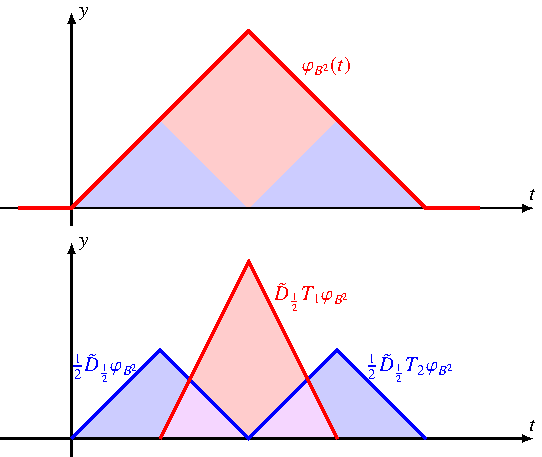
\includegraphics{chapters/6-msa/images/b2skal.pdf}
\caption{Skalierungsrelation für die Funktion $\varphi_{B^2}$
definiert durch \eqref{msa:ortho:beispiel}.
\label{msa:ortho:beispielfig}}
\end{figure}
Die Funktion
\begin{equation}
\varphi_{B^2}(t)
=
\begin{cases}
  t&\qquad 0\le t \le 1\\
2-t&\qquad 1\le t \le 2\\
  0&\qquad \text{sonst}
\end{cases}
\label{msa:ortho:beispiel}
\end{equation}
erfüllt die Skalierungsgleichung
\begin{equation}
\varphi_{B^2}(t)
= 
\frac12\varphi_{B^2}(2t)
+
\varphi_{B^2}(2t-1)
+
\frac12\varphi_{B^2}(2t-2)
\label{eq:skalierung-phi1-proto}
\end{equation}
(siehe Abbildung~\ref{msa:ortho:beispielfig}).
Wir werden in Kapitel~\ref{chapter:spline} zeigen, dass sich daraus ein
geeignetes Mutterwavelet konstruieren lässt.
Eine grundlegende Schwierigkeit, die dabei gelöst werden muss, ist, dass
die Translate $\varphi_{B^2}(t-b)$ für $b\in\mathbb N$ nicht orthonormiert
sind.
Vielmehr ist das Skalarprodukt
\begin{align*}
\langle \varphi_{B^2}, T_{-1}\varphi_{B^2}\rangle
&=
\int_0^1 t\cdot (1-t)\,dt
=
\biggl[
\frac{t^2}{2}-\frac{t^3}{3}
\biggl]_0^1
=
\frac12-\frac13 = \frac16\ne 0.
\end{align*}

% moved here
\rhead{Orthonormalisierung}

In diesem Abschnitt soll daher die folgende Aufgabe gelöst werden.
\begin{aufgabe}
\label{aufgabe:orthonormalisierung}
Gegeben $f\in L^2(\mathbb R)$, konstruiere eine Funktion 
$F\in L^2(\mathbb R)$, die eine Linearkombination von 
Translaten von $f$ ist, also
\[
F(t) = \sum_{k=-\infty}^\infty c_k f(t-k)
\]
und so, dass die Translate von $F$ orthonormiert sind.
\end{aufgabe}

In der linearen Algebra lernt man üblicherweise das Verfahren von
Gram-Schmidt zur Orthonormalisierung einer Basis eines Vektorraumes.
Es beginnt beim ersten Vektor, der nur in seiner Länge verändert wird.
Die folgenden Vektoren werden dann sukzessive modifiziert, so dass sie
auf den bisher behandelten Vektoren senkrecht stehen.
Dieses Vorgehen ist im vorliegenden Fall nicht angebracht, da die
entstehenden Vektoren nicht alle Translate des ersten Vektors sind.

\begin{proof}[Lösung]
In Satz~\ref{satz:msa:orthogonalitaetsbedingung} wurde eine Bedingung
formuliert, mit der man entscheiden kann, ob die Translate einer 
Funktion orthogonal sind.
Für die Fourier-Transformation muss gelten
\[
\mathcal{P}|\hat{F}|^2(\omega)
=
\frac{1}{2\pi}.
\]
Die Funktion 
\[
\Phi(\omega)
=
2\pi\mathcal{P}|\hat{f}|^2(\omega)
\]
ist $2\pi$-periodisch, also auch die Funktion $1/\sqrt{\Phi(\omega)}$.
Sie kann daher in eine Fourier-Reihe
\[
\frac{1}{\sqrt{\Phi(\omega)}}
=
\sum_{k\in\mathbb Z} c_ke^{-ik\omega}
\]
entwickelt werden.
Wir setzen 
\[
\hat{F}(\omega)
=
\frac{1}{\sqrt{\Phi(\omega)}} 
\hat{f}(\omega)
=
\sum_{k\in\mathbb Z} c_ke^{-ik\omega}\hat{f}(\omega).
\]
Offenbar bedeutet dies, dass $F$ eine Linearkombination von Translaten
von $f$ ist.
Wir können aber auch die Orthogonalitätsbedingung verifizieren:
\begin{align*}
\mathcal{P}|\hat{F}|^2
=
\frac{1}{\Phi(\omega)} \mathcal{P}|\hat{f}|^2(\omega)
=
\frac{1}{2\pi}.
\end{align*}
Die Translate der Funktion $F$ sind daher orthonormiert.
\end{proof}

Wenn also
$\Phi(\omega)=\mathcal{P}|\hat{f}(\omega)|^2$ dergestalt ist, dass 
$1/\sqrt{\Phi(\omega}$ eine quadratinterierbare periodische Funktion ist,
dann lassen sich die Translate von $f$ so linear zu $F$ kombinieren, dass die
Translate von $F$ orthonormiert sind.
Die Aufgabe lässt sich also insbesondere dann lösen, wenn $\Phi(\omega)$
keine Nullstellen hat.
Dieser Prozess ersetzt das Gram-Schmidtsche Orthogonalisierungsverfahren
im Falle der Wavelets.





